\documentclass{article}
\usepackage{listings}
\usepackage{color} %red, green, blue, yellow, cyan, magenta, black, white
\definecolor{mygreen}{RGB}{28,172,0} % color values Red, Green, Blue
\definecolor{mylilas}{RGB}{170,55,241}

\usepackage{booktabs}
\usepackage{pgfplots}
\usepackage{pgfplotstable}
\usepackage{movie15}
\usepackage{graphicx}
\usepackage{amsmath}
\usepackage{float}
\usepackage{physics}
\usepackage[colorlinks=true, linkcolor=blue]{hyperref}
\usepackage[english]{babel}
\selectlanguage{english}
\usepackage[utf8]{inputenc}
\usepackage[svgnames]{xcolor}
\usepackage{subfig}
\usepackage{listings}
\usepackage{afterpage}
\pagestyle{plain}
\usepackage{graphicx}

\definecolor{dkgreen}{rgb}{0,0.6,0}
\definecolor{gray}{rgb}{0.5,0.5,0.5}
\definecolor{mauve}{rgb}{0.58,0,0.82}
\definecolor{carrotorange}{rgb}{0.93, 0.57, 0.13}

\lstset{language=C,
    frame=tb,
    backgroundcolor=\color{white},
    commentstyle=\color{dkgreen},
    keywordstyle=\color{blue},
    numbers=none,
    stringstyle=\color{carrotorange},
    basicstyle=\footnotesize,
    breakatwhitespace=false,
    breaklines=true,
    captionpos=b,
    keepspaces=true,
    numbersep=5pt,
    showspaces=false,
    showstringspaces=false,
    showtabs=false,
    tabsize=2,
    language=C
}

\usepackage{here}

\textheight=21cm
\textwidth=17cm
%\topmargin=-1cm
\oddsidemargin=0cm
\parindent=0mm
\pagestyle{plain}

\usepackage{color}
\usepackage{ragged2e}

\global\let\date\relax
\newcounter{unomenos}
\setcounter{unomenos}{\number\year}
\addtocounter{unomenos}{-1}
\stepcounter{unomenos}
\gdef\@date{ Course \arabic{unomenos}}

\begin{document}
\begin{titlepage}
\begin{center}
\vspace*{-1in}
\begin{figure}[htb]
\begin{center}

\includegraphics[width=8cm]{UU_logo.jpg}
\end{center}
\end{figure}

DEPARTMENT OF INFORMATION TECHNOLOGY - \@date\\
\vspace*{0.15in}
HIGH PERFORMANCE PROGRAMMING - LU Decomposition\\
\vspace*{0.3in}
\begin{large}
KIERAN BARBER\\
\end{large}
\vspace*{0.1in}
\rule{80mm}{0.1mm}\\
\vspace*{0.1in}
\begin{large}
Teacher \\
Sverker Holmgren
\end{large}
\end{center}
\end{titlepage}

\newcommand{\CC}{C\nolinebreak\hspace{-.05em}\raisebox{.4ex}{\tiny\bf +}\nolinebreak\hspace{-.10em}\raisebox{.4ex}{\tiny\bf +}}
\def\CC{{C\nolinebreak[4]\hspace{-.05em}\raisebox{.4ex}{\tiny\bf ++}}}

\tableofcontents
\newpage



\section{Introduction}
Lower-Upper (LU) Decomposition is the procedure whereby one factorizes a matrix A as the product of a lower triangular matrix and an upper triangular matrix. This can be viewed as a form of Gaussian elimination. This procedure can be implemented on computers. The use of LU matrices extend to solving systems of linear equations, inverting matrices and computing determinants.
\\\\
There are multiple forms in which we can compute the lower and upper matrices. The most basic of these is to simply compute $A = LU$.
\\\\
Another form of computing the lower and upper matrices is to include partial pivoting. The purpose of this procedure is to negate the issue if any of the diagonal terms are equal to 0. If we have a 0 term, we cannot continue the procedure to build the lower and upper matrices. A more advanced procedure of the above is to use full pivoting where we also rearrange the columns of A.
\\\\
One final form is that of $A = LDU$ where D is a diagonal matrix, which allows for the diagonals of L and U to be set to 1. The benefit of this matrix, is that it can deal with rectangular matrices as well.
\\\\
In the lower triangular matrix, L, all the entries above the diagonal are zero. In the upper triangular matrix, U, all the entries below the diagonal are zero. For example, the decomposition for a $3 \times 3$ matrix can take the following form:
\\\\
\begin{bmatrix}
a_{11} & a_{12} & a_{13}\\
a_{21} & a_{22} & a_{23}\\
a_{31} & a_{32} & a_{33}\\
\end{bmatrix}
=
\begin{bmatrix}
l_{11} & 0 & 0\\
l_{21} & l_{22} & 0\\
l_{31 & l_{32} & l_{33}\\
\end{bmatrix}
\begin{bmatrix}
u_{11} & u_{12} & u_{13}\\
0 & u_{22} & u_{23}\\
0 & 0 & u_{33}\\
\end{bmatrix}
\section{The Problem}
For this problem, we want to write a code that will perform LU decomposition of a matrix A and then optimise the code so that these computations can be done as efficiently as possible. There are several different methods to do this as has been mentioned above, but we will look to implement the particular problem, $A = LU$ decomposition without pivoting.
\section{Solution Method}
To solve this problem, we implement the Doolittle algorithm. As a part of this algorithm, we set the entries of the main diagonal of the lower matrix to 1. We also set the top row of U equal to A.
\\\\
To implement the algorithm, we use a triple for loop. We compute entries for the upper and lower matrix column by column, followed up by row by row. The elements of $L$ and $U$ are set according to
$$U_{ij} = A_{ij} - \sum_{k = 1}^{i - 1}L_{ik}U_{kj};$$
$$L_{ij} = \frac{A_{ij} - \sum_{k=1}^{j-1}L_{ik}U_{kj}}{U_{jj}}.$$
We note that this will fail if the first entry of $U$ is zero.

%-Ofast -march=native
%Store L and U compactly in one matrix.
Now that we have implemented a base case, we look to then parallelize. We cannot, however, parallelize the outer for loop since it has dependencies. The two inner loops can be parallelized without issues.
\\\\
In Version 2, we can improve computation time through using less cache, so more cache is available to perform faster operations. To do this, we see that each of the lower and upper matrix calls in the code can be computed as one matrix given that the boundaries that are set in the for loops hold for each case. This can be viewed in the appendix.
% \newpage
\section{Experiments}
\subsection{Code optimisations}
For a first experiment, a second version of the code was written in order to utilise more of the faster cache. Below are the timings for each version on different optimisation flags.
\begin{center}
    \begin{tabular}{|c|c|c|c|c|}
    \hline
    Version & -O0 & -O3 & -Ofast & -O3 -Ofast -march=native\\
    \hline
    1 & 11.632 & 5.521 & 5.318 & 5.051\\
    \hline
    2 & 18.547 & 4.857 & 4.796 & 4.503\\
    \hline
    \end{tabular}
\end{center}
As can be seen, the optimised code runs faster for all flags aside from -O0. This optimisation can be viewed in the appendix.
\\\\
The next experiment was to test the how the code performed upon increasing the size of the matrix A. Below is a graphic showing how Version 1 compares with Version 2 with the optimised flags -O3, -Ofast and -march=native on both my laptop and the machines at the university.
\\\\
\begin{figure}[htb]
\begin{center}
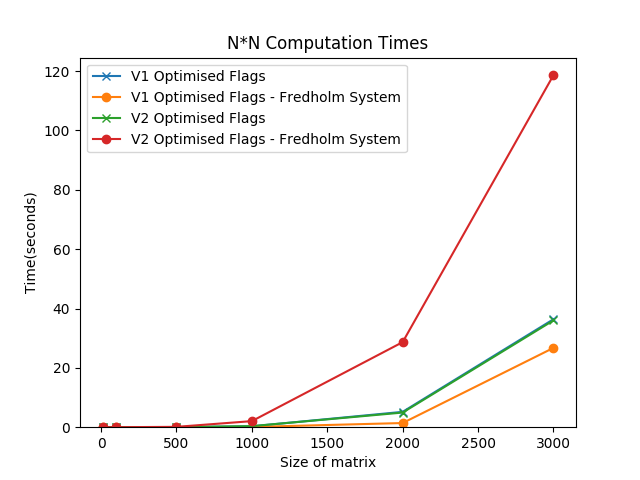
\includegraphics[width=8cm]{NN_comp_times.png}
\caption{Computation Times on an N*N matrix}
\end{center}
\end{figure}
\\\\
We chose to extend the size of the matrix to something that would compute for a reasonable length of time so that we may be able to ascertain what happens as a general trend.
\\\\
From the graphics, we can see that up to around a matrix size of $N = 2000$, everything runs quickly aside from Version 2 with the Fredholm system. The reason behind this is unknown at this moment in time. Computation times start to get much slower at $N = 3000$.
\subsection{Parallelisation}
Another experiment that I wanted to test was the effectiveness of using OpenMP within my code. I inserted a parallelisation above the for loop to compute the lower matrix.
\\\\
\begin{figure}[htb]
\begin{center}
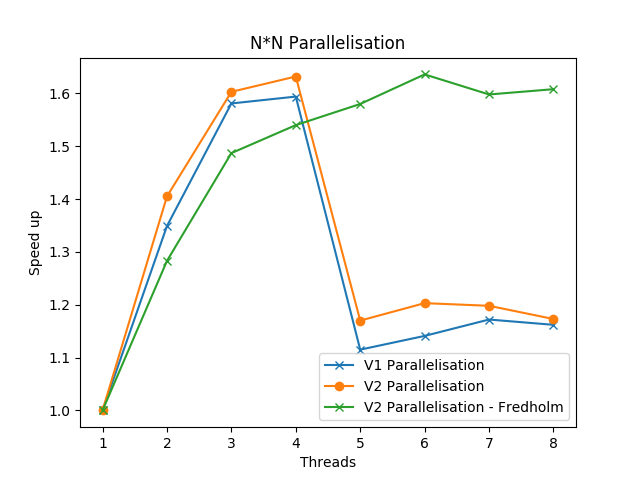
\includegraphics[width=8cm]{NN_speedup.png}
\caption{Speed up graphic: OpenMP}
\end{center}
\end{figure}
\\\\
To test this, I increased the number of threads that I wanted to run the code on each time. As we can see from the graphic, all versions and systems increased with speed up, up until the fourth thread, at which point, my system slowed down again. This could be due to the fact that my laptop runs with four cores and that the system at the university runs with eight. The systems at the university appear to level off in a much smoother manner. However, we can see that the speed up times are nothing near what I would like. So there would appear to be a great deal of optimisations to do.
\subsection{Unsuccessful Optimisations}
I had some other optimisations that I tried but were unsuccessful. First of all, I tried to use some loop unrolling on some of the for loops to get some performance benefit. Unfortunately, this resulted in some failed output with core dumping. There could have been an issue with the number of computations to do and that this being a number not divisible by the number of loops unrolled. Further to this, I also tried to add -funroll-loops into the Makefile. Upon running this, I found no performance benefit, so excluded this.
\\\\
Another attempt at optimisation was to make use of the OpenMP parallelisation option above other for loops. When trying this, I found that adding this to some loops increased computation time. This could be due to the loop trying to access different elements of the array that may not be accessible at that moment in time, so the output matrix gives incorrect results.
\section{Time Complexity}
One final thing that I wanted to look at was how I could model the computation times as N increased.
\begin{figure}[htb]
\begin{center}
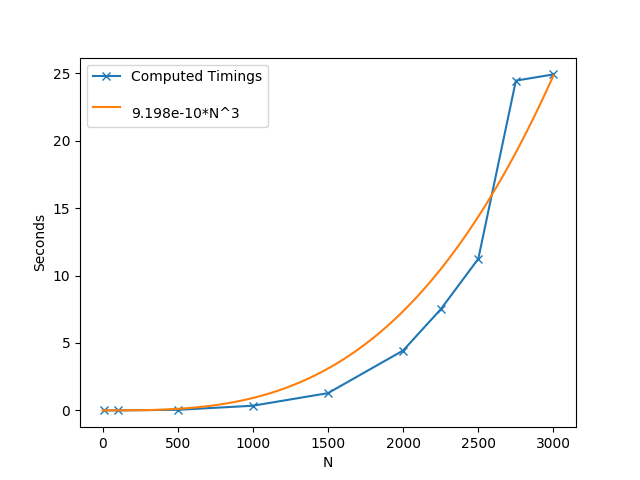
\includegraphics[width=8cm]{model_fit.png}
\caption{Model fit of computation times}
\end{center}
\end{figure}
\\\\
As we can see, the fit we have here is of order $O(N^3)$. This, however, is against advice from literature, so I would expect that with larger size of matrices, this fit will change.
\section{Conclusions}
As expected, with LU decomposition, as the size of the matrix increases faster, the time of the computations increases faster with it. One thing that seems surprising is that the computation times for the Fredholm system are much slower for the second version of the code. \\\\
For future improvements, however, I believe that adjusting the code slightly to be able to more efficiently add parallelisation to speed up the computation time is a must.
\\\\
Further ideas that could be implemented are that of involving other forms of factorization as detailed in the introduction.
\section{References}
\begin{itemize}
    \item Stack
    \item Course Material
    \item Wikipedia
\end{itemize}
\newpage
\section{Code}
\begin{center}
    Version 1
\end{center}

\begin{lstlisting}{langauge=C}
for(j = 0; j < n; j++) {
    U[0][j] = A[0][j];
}

for(i = 0; i < n; i++) {
    L[i][i] = 1;
}

for(i = 1; i < n; i++) {
    L[i][0] = A[i][0]/U[0][0];
}

for(j = 1; j < n; j++) {
    for(i = 1; i <= j; i++) {
        for(k = 0; k <= i - 1; k++) {
            sum = sum + (L[i][k] * U[k][j]);
        }
        U[i][j] = A[i][j] - sum;
        sum = 0;
    }

    #pragma omp parallel for
    for(i = j + 1; i < n; i++) {
        for(k = 0; k <= j - 1; k++) {
            sum = sum + (L[i][k] * U[k][j]);
        }
        L[i][j] = (A[i][j] - sum) / U[j][j];
        sum = 0;
    }
}
\end{lstlisting}
\begin{center}
    Version 2
\end{center}
\begin{lstlisting}
for(j = 0; j < n; j++) {
    LU[0][j] = A[0][j];
}

for(i = 1; i < n; i++) {
    LU[i][0] = A[i][0]/LU[0][0];
}

for(j = 1; j < n; j++) {
    for(i = 1; i <= j; i++) {
        for(k = 0; k <= i - 1; k++) {
            sum = sum + (LU[i][k] * LU[k][j]);
        }
        LU[i][j] = A[i][j] - sum;
        sum = 0;
    }
#pragma omp parallel for
    for(i = j + 1; i < n; i++) {
        for(k = 0; k <= j - 1; k++) {
            sum = sum + (LU[i][k] * LU[k][j]);
        }
        LU[i][j] = (A[i][j] - sum) / LU[j][j];
        sum = 0;
    }
}
\end{lstlisting}
\section{CPU Configuration}
\subsection{Laptop}
\begin{verbatim}
Architecture:        x86_64
CPU op-mode(s):      32-bit, 64-bit
Byte Order:          Little Endian
CPU(s):              8
On-line CPU(s) list: 0-7
Thread(s) per core:  2
Core(s) per socket:  4
Socket(s):           1
NUMA node(s):        1
Vendor ID:           GenuineIntel
CPU family:          6
Model:               142
Model name:          Intel(R) Core(TM) i5-8250U CPU @ 1.60GHz
Stepping:            10
CPU MHz:             700.041
CPU max MHz:         3400,0000
CPU min MHz:         400,0000
BogoMIPS:            3600.00
Virtualization:      VT-x
L1d cache:           32K
L1i cache:           32K
L2 cache:            256K
L3 cache:            6144K
NUMA node0 CPU(s):   0-7

(Ubuntu 7.4.0-1ubuntu1~18.04.1) 7.4.0

\end{verbatim}\textbf{}
\newpage
\subsection{Fredholm}
\begin{verbatim}
    Architecture:        x86_64
CPU op-mode(s):      32-bit, 64-bit
Byte Order:          Little Endian
CPU(s):              16
On-line CPU(s) list: 0-15
Thread(s) per core:  2
Core(s) per socket:  4
Socket(s):           2
NUMA node(s):        2
Vendor ID:           GenuineIntel
CPU family:          6
Model:               26
Model name:          Intel(R) Xeon(R) CPU           E5520  @ 2.27GHz
Stepping:            5
CPU MHz:             1600.202
CPU max MHz:         2267,0000
CPU min MHz:         1600,0000
BogoMIPS:            4533.84
Virtualization:      VT-x
L1d cache:           32K
L1i cache:           32K
L2 cache:            256K
L3 cache:            8192K
NUMA node0 CPU(s):   0-3,8-11
NUMA node1 CPU(s):   4-7,12-15

\end{verbatim}
\end{document}
